% BU ECE template for MS thesis and PhD dissertation.
%
%==========================================================================%
% MAIN PREAMBLE 
%==========================================================================%
\documentclass[12pt,letterpaper]{report}          % Single-sided printing for the library
%\documentclass[12pt,twoside]{report} % Double-sided printing
\usepackage[intlimits]{amsmath}
\usepackage{amsfonts,amssymb}
\DeclareSymbolFontAlphabet{\mathbb}{AMSb}
%\usepackage{natbib}
\usepackage{apalike}
\usepackage{float}
\usepackage[bf]{caption}       
\setcaptionmargin{0.5in}
\usepackage{fancyhdr}
%\usepackage{fancyheadings}
\usepackage{fancybox}
\usepackage{ifthen}
\usepackage{bu_ece_thesis}
\usepackage{url}
\usepackage{lscape,afterpage}
\usepackage{xspace}
\usepackage{epstopdf} 
\usepackage{subfig}
%==========================================================================%
%%% graphicx and pdf creation
\usepackage{graphicx}
\usepackage{appendix}
%\usepackage{psfrag}
%\DeclareGraphicsExtensions{.eps}   % extension for included graphics
%\usepackage{thumbpdf}              % thumbnails for ps2pdf
%\usepackage[ps2pdf,                % hyper-references for ps2pdf
%bookmarks=true,%                   % generate bookmarks ...
%bookmarksnumbered=true,%           % ... with numbers
%hypertexnames=false,%              % needed for correct links to figures !!!
%breaklinks=true,%                  % breaks lines, but links are very small
%linkbordercolor={0 0 1},%          % blue frames around links
%pdfborder={0 0 112.0}]{hyperref}%  % border-width of frames 
%                                   % will be multiplied with 0.009 by ps2pdf
%\hypersetup{
%  pdfauthor   = {Joe Graduate <joe.graduate@bu.edu>},
%  pdftitle    = {dissertation.pdf},
%  pdfsubject  = {doctoral dissertations},
%  pdfkeywords = {mathematics, science, technology},
%  pdfcreator  = {LaTeX with hyperref package},
%  pdfproducer = {dvips + ps2pdf}
%}
%==========================================================================%
% customized commands can be placed here
%\newcommand{\figref}[1]{Figure~\ref{#1}}
%\newcommand{\chapref}[1]{Chapter~\ref{#1}}
%\newcommand{\latex}{\LaTeX\xspace}
%==========================================================================%

%==========================================================================%
% BEGIN
%==========================================================================%
\begin{document}

% The preliminary pages

% This file contains all the necessary setup and commands to create
% the preliminary pages according to the buthesis.sty option.

\title{Query planning for Stream Processing}

\author{Apoorva Tamaskar}

% Type of document prepared for this degree:
%   1 = Master of Science thesis,
%   2 = Doctor of Philisophy dissertation.
%   3 = Master of Science thesis and Doctor of Philisophy dissertation.
\degree=2

\prevdegrees{	M.Sc.,  University of Glasgow, 2018\\
B.Sc. Hons, Chennai Mathematical Institute , 2017}

\department{Department of Computer Science}

% Degree year is the year the diploma is expected, and defense year is
% the year the dissertation is written up and defended. Often, these
% will be the same, except for January graduation, when your defense
% will be in the fall of year X, and your graduation will be in
% January of year X+1
\defenseyear{2020}
\degreeyear{2020}

% For each reader, specify appropriate label {First, Second, Third},
% then name, and title. IMPORTANT: The title should be:
%   "Professor of Electrical and Computer Engineering",
% or similar, but it MUST NOT be:
%   Professor, Department of Electrical and Computer Engineering"
% or you will be asked to reprint and get new signatures.
% Warning: If you have more than five readers you are out of luck,
% because it will overflow to a new page. You may try to put part of
% the title in with the name.
\reader{First}{Kia Teymourian, PhD}{Assistant Professor of computer science}
\reader{Second}{Eugene Pinsky, PhD}{Assistant Professor of Computer Science}
\reader{Third}{Reza Rawassizadeh, PhD}{Associate Professor of Computer Science }

% The Major Professor is the same as the first reader, but must be
% specified again for the abstract page. Up to 4 Major Professors
% (advisors) can be defined. 
\numadvisors=1
\majorprof{Kia Teymourian, PhD}{{Assistant Professor of computer science}}
%\majorprofc{First M. Last, PhD}{{Professor of Astronomy}}
%\majorprofd{First M. Last, PhD}{{Professor of Biomedical Engineering}}

%%%%%%%%%%%%%%%%%%%%%%%%%%%%%%%%%%%%%%%%%%%%%%%%%%%%%%%%%%%%%%%%  

%                       PRELIMINARY PAGES
% According to the BU guide the preliminary pages consist of:
% title, copyright (optional), approval,  acknowledgments (opt.),
% abstract, preface (opt.), Table of contents, List of tables (if
% any), List of illustrations (if any). The \tableofcontents,
% \listoffigures, and \listoftables commands can be used in the
% appropriate places. For other things like preface, do it manually
% with something like \newpage\section*{Preface}.

% This is an additional page to print a boxed-in title, author name and
% degree statement so that they are visible through the opening in BU
% covers used for reports. This makes a nicely bound copy. Uncomment only
% if you are printing a hardcopy for such covers. Leave commented out
% when producing PDF for library submission.
%\buecethesistitleboxpage

% Make the titlepage based on the above information.  If you need
% something special and can't use the standard form, you can specify
% the exact text of the titlepage yourself.  Put it in a titlepage
% environment and leave blank lines where you want vertical space.
% The spaces will be adjusted to fill the entire page.
\maketitle
\cleardoublepage

% The copyright page is blank except for the notice at the bottom. You
% must provide your name in capitals.
\copyrightpage
\cleardoublepage

% Now include the approval page based on the readers information
\approvalpage
\cleardoublepage

% Here goes your favorite quote. This page is optional.
\newpage
%\thispagestyle{empty}

% \vspace{0.7in}
%
% \noindent
% [The descent to Avernus is easy; the gate of Pluto stands open night
% and day; but to retrace one's steps and return to the upper air, that
% is the toil, that the difficulty.]

\cleardoublepage

% The acknowledgment page should go here. Use something like
% \newpage\section*{Acknowledgments} followed by your text.
\newpage
\section*{\centerline{Acknowledgments}}
Over the course of writing this thesis, I have received lots of support and assistance.\\
First of all, I would like to thank my supervisor, Professor Kia Teymourian, who guided me and helped me formulate the research question, provided me with sources and methodology. Your insightful feedback pushed me to sharpen my thought process and helped me elevate the quality of my work.\\
I would like to thank the administrative staff at MET college, especially Ronette Lyle and the BU ISSO team who helped me through the administrative process.\\
I would like to acknowledge my friends and colleagues at Boston University for their wonderful feedback and discussions.\\
Also, I would like to thank my parents and my brother for their wise counsel, an empathetic ear and for always being there for me.
\vskip 1in

\noindent
Apoorva Tamaskar\\
Metropolitan College

\cleardoublepage

% The abstractpage environment sets up everything on the page except
% the text itself.  The title and other header material are put at the
% top of the page, and the supervisors are listed at the bottom.  A
% new page is begun both before and after.  Of course, an abstract may
% be more than one page itself.  If you need more control over the
% format of the page, you can use the abstract environment, which puts
% the word "Abstract" at the beginning and single spaces its text.

\begin{abstractpage}
% ABSTRACT
Our increasingly connected world has resulted in the generation of many data streams. With the rise in network traffic and increased interconnectivity, analyzing data and extracting key information has become challenging. Executing queries to extract insights from the data is now more essential than ever to make quick and efficient decisions. The flexibility of reinforcement learning, along with strong prediction properties, and precise mathematical model of Deep neural networks combined results in the technique called Deep reinforcement learning which can be a robust and promising method to reduce query processing times. While there is a lot of research on query optimization on data streams, none showcase the use of Deep reinforcement learning. The continuous nature of datastreams renders the conventional approaches inapplicable, due to increased processing time. The method implemented in this thesis is generic enough so that it applies to a wide range of data streams and queries to optimize the query processing time. The goal of this study is to act as a proof of concept. The thesis explores the use of deep reinforcement learning on a query from Linear road benchmark data. The proposed method is demonstrated to be effective in picking optimal query plan, and reducing the query execution time. We hope the work in this thesis encourages others to work on the development of a robust and more generalized system, capable of optimizing any query on any data stream.


\end{abstractpage}
\cleardoublepage

% Now you can include a preface. Again, use something like
% \newpage\section*{Preface} followed by your text

% Table of contents comes after preface
\tableofcontents
\cleardoublepage

% If you do not have tables, comment out the following lines
\newpage
\listoftables
\cleardoublepage

% If you have figures, uncomment the following line
\newpage
\listoffigures
\cleardoublepage

% List of Abbrevs is NOT optional (Martha Wellman likes all abbrevs listed)
\chapter*{List of Abbreviations}

{\bf The list below must be in alphabetical order as per BU library instructions or it will be returned to you for re-ordering.}

\begin{center}
  \begin{tabular}{lll}
    \hspace*{2em} & \hspace*{1in} & \hspace*{4.5in} \\
    CAD  & \dotfill & Computer-Aided Design \\
    CO   & \dotfill & Cytochrome Oxidase \\
    DOG  & \dotfill & Difference Of Gaussian (distributions) \\
    FWHM & \dotfill & Full-Width at Half Maximum \\
    LGN  & \dotfill & Lateral Geniculate Nucleus \\
    ODC  & \dotfill & Ocular Dominance Column \\
    PDF  & \dotfill & Probability Distribution Function \\
    $\mathbb{R}^{2}$  & \dotfill & the Real plane \\
  \end{tabular}
\end{center}
\cleardoublepage

% END OF THE PRELIMINARY PAGES

\newpage
\endofprelim
        
\cleardoublepage

% -------------------------------------
% CHAPTER 1: INTRODUCTION
% -------------------------------------
\chapter{Introduction}
\label{chapter:Introduction}
\thispagestyle{myheadings}

\section{Motivation}
\label{sec:Motivation}
Hi
\section{Problem at hand}
\label{sec:Problem at hand}
Hello
\section{Structure of thesis}
\label{sec:Structure of thesis}
Works
\section{Conclusion}
\label{sec:Conclusion}
Nope

\cleardoublepage

% -------------------------------------
% CHAPTER 2: THE BODY OF THESIS
% -------------------------------------
\chapter{Body of my thesis}
\label{chapter:body}
\thispagestyle{myheadings}

% set this to the location of the figures for this chapter. it may
% also want to be ../Figures/2_Body/ or something. make sure that
% it has a trailing directory separator (i.e., '/')!
\graphicspath{{2_Body/Figures/}}

\section{Some results}
\label{sec:results}

Here goes all the important stuff, likely with a lot of graphics like this:

\begin{figure}[htb]
  \begin{minipage}[t]{0.49\linewidth}\centering
    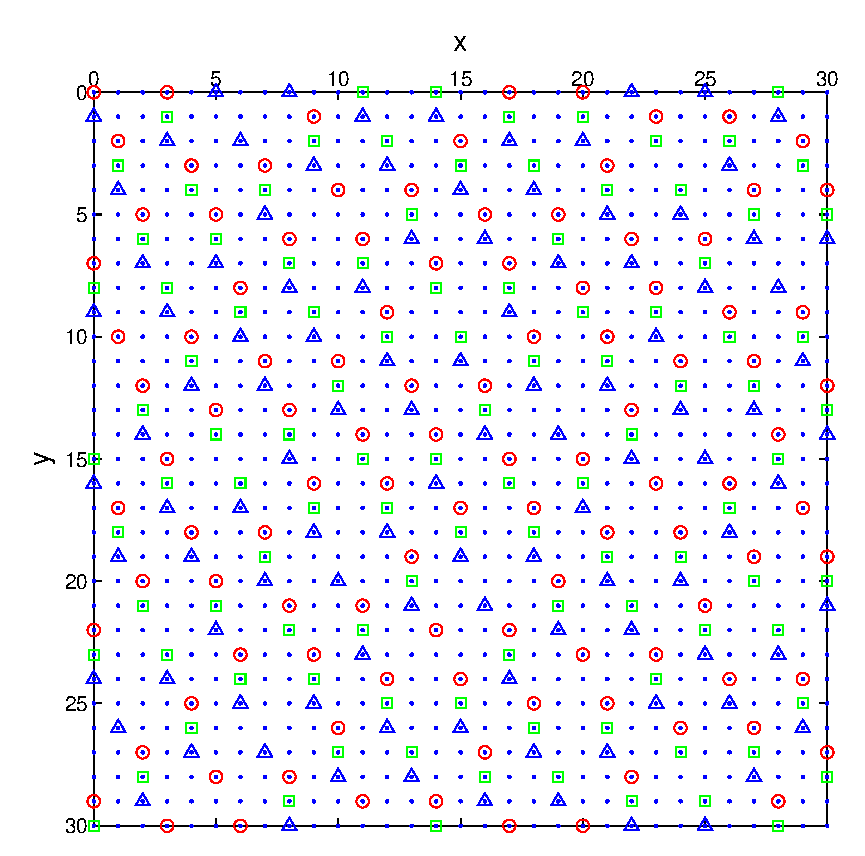
\includegraphics[width=7cm]{figure_sampling_view1.eps}
    \medskip
    \centerline{(a)}
  \end{minipage}\hfill
  \begin{minipage}[t]{0.49\linewidth}\centering
    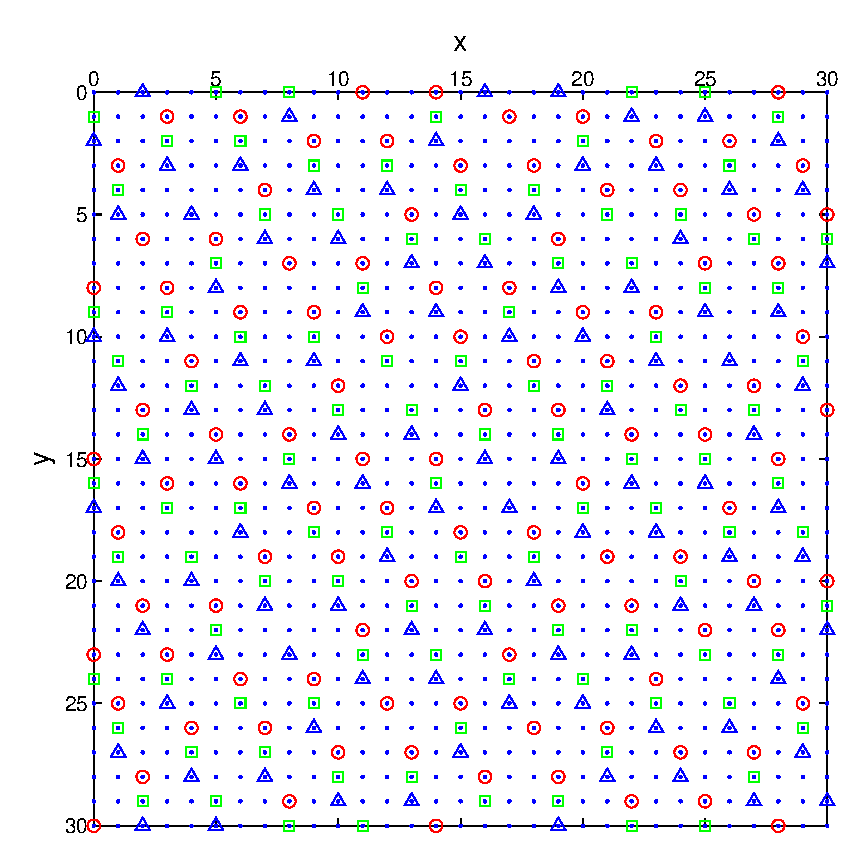
\includegraphics[width=7cm]{figure_sampling_view2.eps}
    \medskip
    \centerline{(b)}
  \end{minipage}
  \caption{Assignment of single-view intensities to RGB components: (a) view
    \#1; and (b) view \#2. }
  \label{fig:Sampling}
\end{figure}

You will also be using a lot of citations. Here is the format required in the dissertation: \cite{lamport1985:latex},\cite{Debr01}.

In all likelihood, you will need to insert tables. See one example on the next page.
\clearpage

\begin{table}[h]
	\caption{Absolute disparity error per pixel for the test data from
		Fig.~\ref{fig:Sampling} and different parameter values. In each experiment one
		parameter is adjusted while other parameters are unchanged.} 
	\centering
	\begin{minipage}[b]{0.30\linewidth}
		\centerline{$\eta=6000$, $\mu=2000$}\smallskip
		\centering
		\begin{tabular}{ccc}
			\hline
			$K$ & $u_1$ & $u_2$\\
			\hline
			3   & 0.52 &0.46\\
			7   & 0.47 &0.43\\
			10  & 0.35 &0.36\\
			12  & 0.37 &0.36\\
			\hline
		\end{tabular}
	\end{minipage}
	%
	\begin{minipage}[b]{0.34\linewidth}
		\centerline{$K=10$, $\mu=2000$}\smallskip
		\centering
		\begin{tabular}{ccc}
			\hline
			$\eta$ & $u_1$ & $u_2$\\
			\hline
			1000&0.54& 0.45\\
			3000&0.43& 0.40\\
			6000&0.35& 0.36\\
			9000&0.37& 0.37\\
			\hline
		\end{tabular}
	\end{minipage}
	%
	\begin{minipage}[b]{0.32\linewidth}
		\centerline{$K=10$, $\eta=6000$}\smallskip
		\centering
		\begin{tabular}{ccc}
			\hline
			$\mu$ & $u_1$ & $u_2$\\
			\hline
			100 &1.00&1.16\\
			1000&0.53&0.47\\
			2000&0.35&0.36\\
			3000&0.44&0.43\\
			\hline
		\end{tabular}
	\end{minipage}
	%
	\label{tab:Parameters}
\end{table}

Of course, there must be a Table of Contents at the beginning of the thesis.
\cleardoublepage

% -------------------------------------
% CHAPTER 3: CONCLUSION
% -------------------------------------
\chapter{Conclusion and Further work}
\label{chapter:Conclusion_and_further_work}
\thispagestyle{myheadings}

% set this to the location of the figures for this chapter. it may
% also want to be ../Figures/2_Body/ or something. make sure that
% it has a trailing directory separator (i.e., '/')!
\graphicspath{}

\section{Conclusion}
The goal of this thesis is to act as a proof of concept for the application of Deep Reinforcement Learning for optimization of query processing on streams.\\
Say, for a particular window of data the size of SegVol $=x$ and size of SegAvgSpeed $=y$, due to the query used in the experiments, the number of operations required to execute the query lie between $[x*y,4*x*y]$. The worst and best possible cases can both arise in the same window depending on the order used and the data in the query.\\
Of the $24$ possible operation orders, we were able to predict the optimal order of operations around $48\%$ cases, reducing the number of operations to around $38\%$ of the worst observed(which is better than the actual worst).
\begin{center}
$x*y \leq$ optimal $\leq$ predicted $\leq$ worst observed $\leq 4*x*y$
\end{center}

\section{Further Work}
This thesis proposed a method for optimization of query execution on data stream and provided a demo implementation for experimentation. There are still many areas which can be improved and developed further.

\subsection{Data Generation}
As shown in chapter $5$, the data generated is highly biased. A source producing more diverse data and a query on that may lead to more interesting results. Real world data stream can be used to get better variety in the data and take input via different methods.

\subsection{Data Storage}
Currently, for executing the query, we store data in vectors where as SQL uses B-trees, a change like this can impact the time required for query execution and then lead to a different learnd model if the time of execution is used as reward.\\
On a further note data storage on systems like AWS S3 buckets, filesystems like Hadoop, hdfs and others can lead to changes in time of execution as well.

\subsection{Features extraction}
The current features only include the entropy of the columns and the size of the tables. Whereas in traditional SQL with a static database(relatively) a lot more features of generally extracted. Better starting feature can perhaps lead to a better results. 

\subsection{Deep Reinforcement Learning}
The Deep reinforcement learning model used was rather simplfied due to the less number of moves and convert the game into a single step game. Further intensive state, action and reward tuples can be constructed to get better intermediate rewards and policies. 

\subsection{Integration} 
The learnt DQN can be integrated with an actual stream processing system and tested in full for scalability, reliability and more. Need to note that there is a speedup by number of operations, the runtime due to various other network constraints might have a different result. 

\cleardoublepage

%\appendix
\begin{appendices}
\chapter{Proof of xyz}
\label{appendix}
\thispagestyle{myheadings}

This is the appendix.
\end{appendices}
%==========================================================================%
% Bibliography
\newpage
\singlespace
\bibliographystyle{apalike}

% each subdirectory can have its own BiBTeX file
\bibliography{thesis}
\cleardoublepage

%==========================================================================%
% Curriculum Vitae
\addcontentsline{toc}{chapter}{Curriculum Vitae}

\thispagestyle{empty}

\begin{center}
{\LARGE {\bf CURRICULUM VITAE}}\\
\vspace{0.5in}
{\large {\bf Joe Graduate}}
\end{center}

Basically, this needs to be worked out by each individual, however the same format, margins, typeface, and type size must be used as in the rest of the dissertation. 
 

%==========================================================================%
\end{document}
